\documentclass[blue,normal,cn]{elegantnote}
\usepackage{pdfpages}

\begin{document}
	

\includepdf[pages={1}]{NETWORK.pdf}
	
\section{实验介绍}
\subsection{实验内容和实验目的}
本次实验内容:
\begin{enumerate}
	\item 捕获在连接Internet过程中产生的网络层分组:DHCP分组,ARP分组,IP数据分组,ICMP分组。
	\item 分析各种分组的格式,说明各种分组在建立网络连接过程中的作用。
	\item 分析IP数据分组分片的结构。通过本次实验了解计算机上网的工作过程,学习各种网络层分组的格式及其作用,理解长度大于1500字节IP数据组分片传输的结构。
	
\end{enumerate}
\subsection{实验重点}
重点分析网络层分组的格式,掌握各种分组在网络通信中的应用,了解整个上网的工作过程。发送ICMP分组,并分析其结构和功能。制作长度大于1500字节的IP数据分组,发送并分析其分片传输的过程。
\subsection{实验环境}
\begin{itemize}
	\item 操作系统\ Windows 10
	\item 网卡型号\ Realtek RTL8822BE
\end{itemize}

使用的 Wireshark 软件版本等在此不表。

\section{分析网络层分组结构}
\subsection{DHCP 分组}
通过断网重连的方式,捕获如图~\ref{DHCP_raw}~ 所示的 DHCP 分组。

\begin{figure}[!htbp]
	\centering
	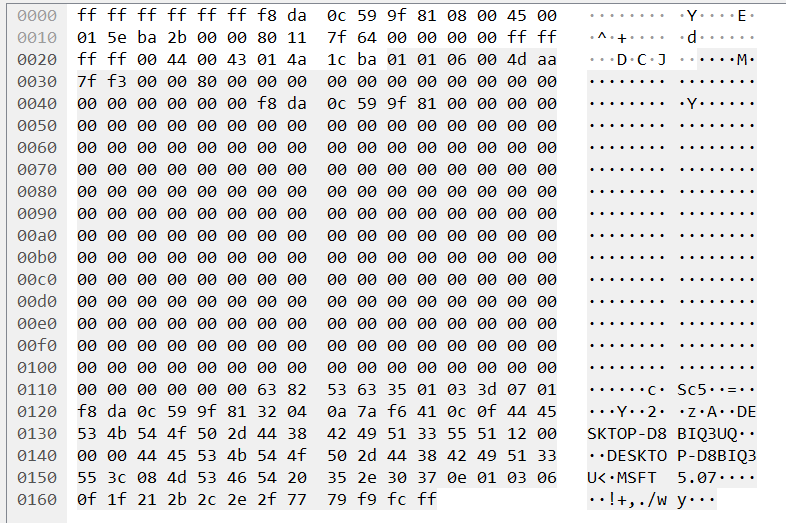
\includegraphics[width=.7\textwidth]{DHCP_raw.png}
	\caption{DHCP 分组}
	\label{DHCP_raw}
\end{figure}

Wireshark 对该分组的解析见图 ~\ref{DHCP_result}~。

\begin{figure}[!htbp]
	\centering
	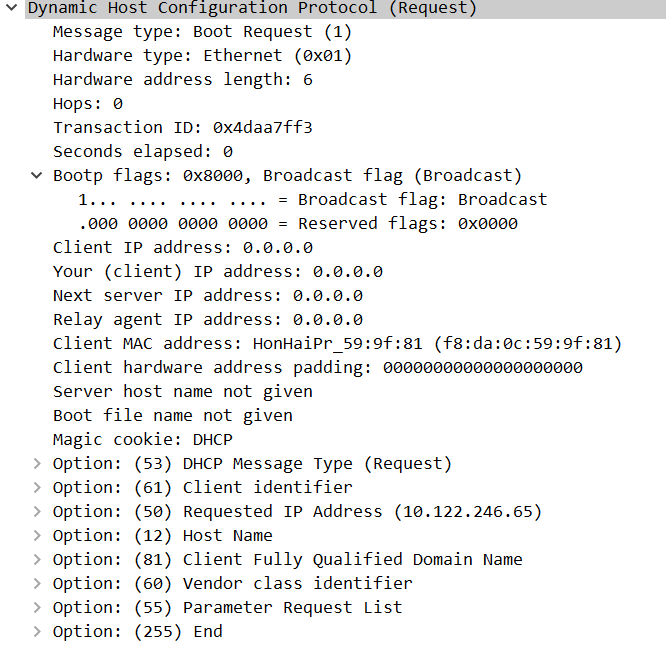
\includegraphics[width=.7\textwidth]{DHCP_result.png}
	\caption{Wireshark 对于 DHCP 分组的解析}
	\label{DHCP_result}
\end{figure}

由此可见,计算机以广播的形式发送了一个 DHCP \textbf{request} 信息,并在该信息中以\href{https://tools.ietf.org/html/rfc2132#section-9.1}{拓展}的形式(Option code: 50)请求 IP 地址 \textbf{10.122.246.65}。此时如果该地址未被分配,服务器会直接将该地址分配给我们,否则会重新分配新的 IP 地址。

\subsubsection{上网流程}
当我们的计算机连接上 \textbf{BUPT-portal} 热点时,首先会广播 \textbf{DHCP request} 包,当服务器回应 IP 地址后,即可正常上网。 

\subsection{IP 数据分组}
任选一包,其 IP 包头数据见图~\ref{IP_raw}~。

\begin{figure}[!htbp]
	\centering
	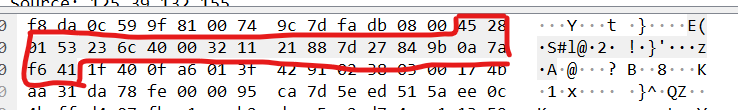
\includegraphics[width=.7\textwidth]{IP_raw.png}
	\caption{IP 包头}
	\label{IP_raw}
\end{figure}

Wireshark 对其分析见图~\ref{IP_result}~。

\begin{figure}[!htbp]
	\centering
	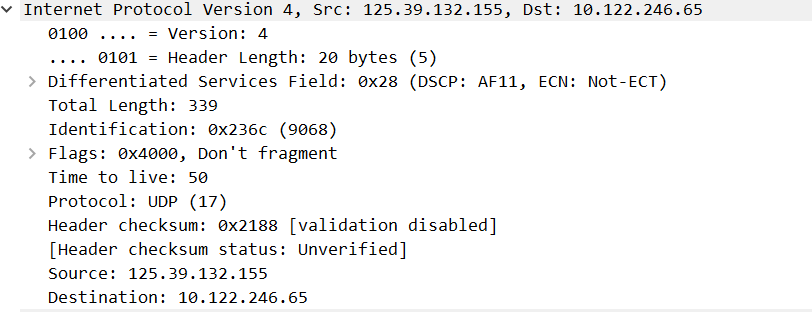
\includegraphics[width=.7\textwidth]{IP_result.png}
	\caption{IP 包头的解析结果}
	\label{IP_result}
\end{figure}

\subsection{ICMP 数据分组}
使用 ping 指令发送 ICMP 分组,数据见图~\ref{ICMP_raw}~。

\begin{figure}[!htbp]
	\centering
	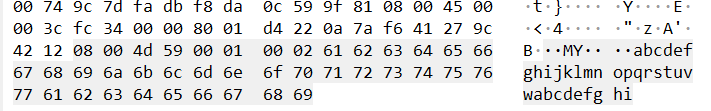
\includegraphics[width=.7\textwidth]{ICMP_raw.png}
	\caption{ICMP 分组}
	\label{ICMP_raw}
\end{figure}

Wireshark 对其的解码结果见图~\ref{ICMP_result}~。

\begin{figure}[!htbp]
	\centering
	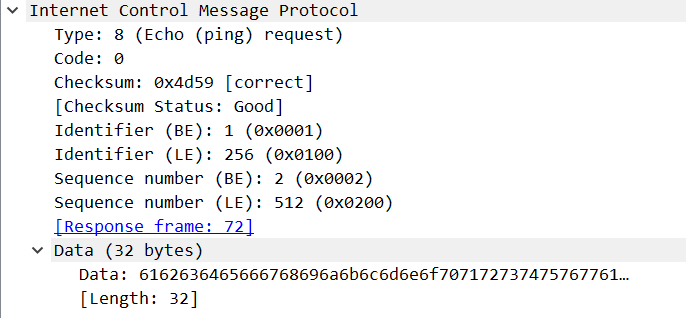
\includegraphics[width=.7\textwidth]{ICMP_result.png}
	\caption{ICMP 包的解析结果}
	\label{ICMP_result}
\end{figure}

\subsection{分片的 IP 数据分组}
通过 ``'ping -l 8000 10.3.9.5' 指令造出一个长度为 8000 字节的分组并使用 Wireshark 捕获,共捕获到如图~\ref{fIP_packets}~所示的分组。

\begin{figure}[!htbp]
	\centering
	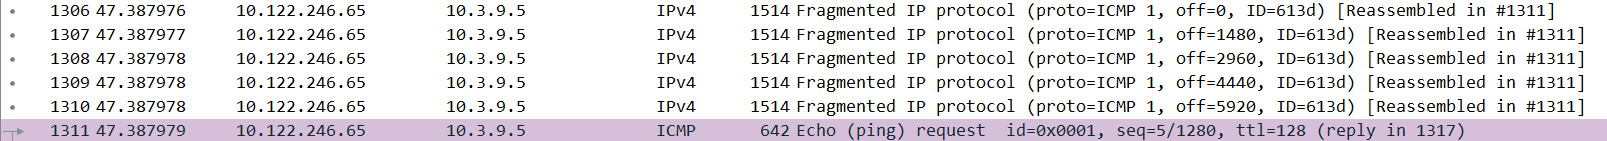
\includegraphics[width=.7\textwidth]{fIP_packets.png}
	\caption{分片的 IP 包}
	\label{fIP_packets}
\end{figure}

现在给出其中一个分片的解析结果,见图片~\ref{fIP_results}~。

\begin{figure}[!htbp]
	\centering
	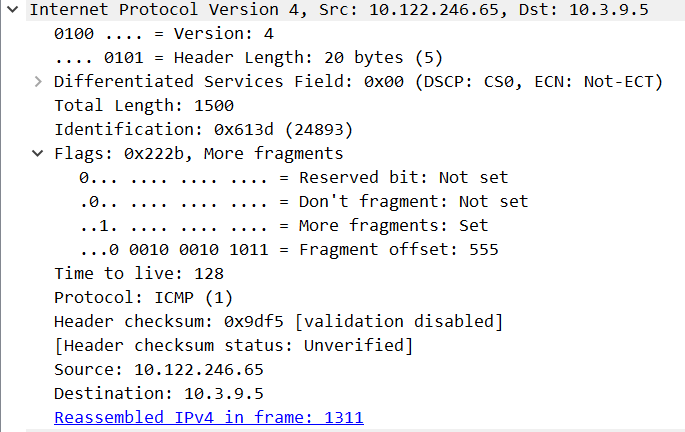
\includegraphics[width=.7\textwidth]{fIP_results.png}
	\caption{解析结果}
	\label{fIP_results}
\end{figure}

几个分组的 IP 头部分只有校验和和偏移量部分不同,其余部分完全一致。在最后一个分组内,``More fregments'' 部分被置为 0,表示不再有新的分片。全套分组大小为 8000 个字节的 IP 数据再加上 8 字节的 ICMP 部分,共 8008 字节。

\section{结论与心得}
该实验共花费了大约两个小时的时间来完成。并未发现任何问题。

通过该实验,我对各种数据包的格式有了更深的理解,并对 IP 的分片机制有了新的认知。

\end{document}